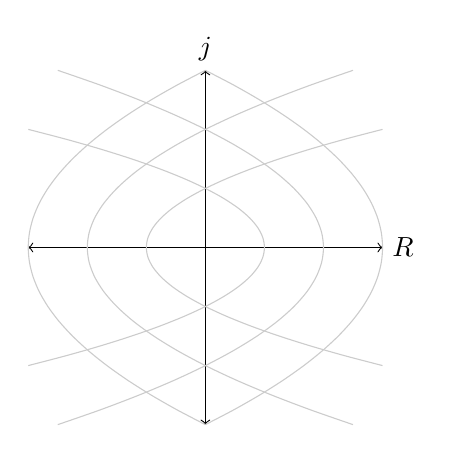
\begin{tikzpicture}[scale= 0.75]
        \draw[<->] (-3,0)--(3,0) node[right] {$R$};
        \draw[<->] (0,-3)--(0,3) node[above]{$j$};
        \draw[rotate=90,thin,gray!40]   plot[smooth,domain=-2:2] (\x, {((\x)^2)-1});
        \draw[rotate=90,thin,gray!40]   plot[smooth,domain=-3:3] (\x, {((\x)^2)/2-2});
        \draw[rotate=90,thin,gray!40]   plot[smooth,domain=-3:3] (\x, {((\x)^2)/3-3});
        \draw[rotate=-90,thin,gray!40]   plot[smooth,domain=-2:2] (\x, {((\x)^2)-1});
        \draw[rotate=-90,thin,gray!40]   plot[smooth,domain=-3:3] (\x, {((\x)^2)/2-2});
        \draw[rotate=-90,thin,gray!40]   plot[smooth,domain=-3:3] (\x, {((\x)^2)/3-3});
\end{tikzpicture}
\caption*{Plano complejo $w$}